\documentclass[12pt,a4paper]{report}
\usepackage[utf8]{inputenc}
%\usepackage[T1]{fontenc}
\usepackage{amsmath}
\usepackage{amsfonts}
\usepackage{amssymb}
\usepackage{graphicx}
\usepackage{physics}
\usepackage{cite}
\usepackage{caption}
\usepackage{subcaption}
%\usepackage{hyperref}
\usepackage{comment}
\usepackage{epsfig}
\usepackage{latexsym}
\usepackage{color} 
%\linespread{1.2}
%\usepackage[a4paper,top=3cm,bottom=3cm,left=3cm,right=3cm]{geometry}

\title{Thesis Work: Ergotropy and Quantum Phase Transitions }
\author{}
\begin{document}
   \maketitle
\tableofcontents{}

   
\chapter{Introduction}
\chapter{Ergotropy and related measures}
\section{Ergotropy}
\section{Max-Ergotropy}
\section{Other Measures}
\chapter{Quantum Phase Transitions}
\section{Heisenberg Models}
\subsection{Transverse Field Ising Model}
\subsection{XY model}
\subsection{XXZ Model}
\chapter{Analitical Calculations}
\section{The XY Model ground state}
Correlation Matrix Derivation
\clearpage
\subsection{One Site}

There are only two Majorana fermions: $\check{a}_1$ and $\check{a}_2$.\\
The one-site Hamiltonian is $-\frac{\lambda}{2}\sigma^z$\\
We write all the correlators in the form $\delta_{m n}+i\Gamma_{m n}$:
\begin{equation}
	\langle\check{a}_{m} \check{a}_{n}\rangle= \left[\begin{array}{cc}
		1 & 0 \\
		0 & 1
	\end{array}\right]+i\left[\begin{array}{cc}
		0 & g_0 \\
		-g_0 & 0
	\end{array}\right]
\end{equation}
$\Gamma$ is already in the block diagonal form.\\
The density matrix $\rho_1$ has eigenvalues:
\begin{equation}
	p_1=(1+g_0)/2 \quad p_2=(1-g_0)/2
\end{equation}\\
With $g_0$:
\begin{equation}
	g_0=\frac{1}{2 \pi} \int_{0}^{2 \pi} d \phi \frac{\lambda-\cos \phi+i \sin \phi}{|\lambda-\cos\phi +i  \sin \phi|}=\frac{1}{2 \pi} \int_{0}^{2 \pi} d \phi \frac{\lambda-\cos \phi}{\sqrt{(\lambda-\cos\phi)^2 +  \sin^2 \phi}}
\end{equation}
\begin{figure}[h!]
	\centering
	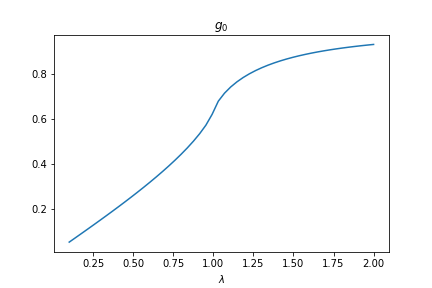
\includegraphics[width=0.7\linewidth]{g0}
	\caption{}
	\label{fig:g0}
\end{figure}\\
\begin{figure}[h!]
	\centering
	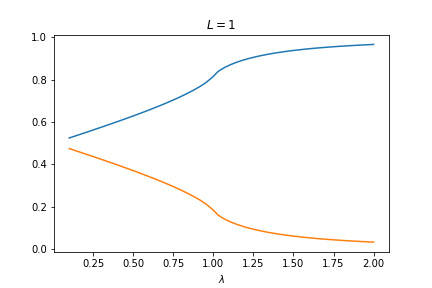
\includegraphics[width=0.7\linewidth]{L1_lambda}
	\caption{Eigenvalues of one-site density matrix}
	\label{fig:l1lambda}
\end{figure}\\
From the eigenvalues we can already calculate something:
\begin{itemize}
	\item Purity: 
	
	\begin{equation}
		\mathfrak{P}(1)=\sum_{i}\left(p_{i}\right)^{2}=\frac{1+g_0^2}{2}
	\end{equation}
	\item Max-Ergo:
	
	\begin{equation}
		\mathcal{M}(1)=2 \sum_{i=1}^{D / 2}\left(p_{i}^{(\downarrow)}-p_{D-i+1}^{(\downarrow)}\right)\left|\epsilon_{i}^{(\uparrow)}\right|=2(p_1-p_2)\abs{e_1}=2g_0\abs{\frac{\lambda}{2}}
	\end{equation}
	\item Rescaled-Max-Ergo
	\begin{equation}
		\mathfrak{M}(\mathcal{I})=g_0
	\end{equation}	
	
\end{itemize}
\begin{figure}[h]
	\centering
	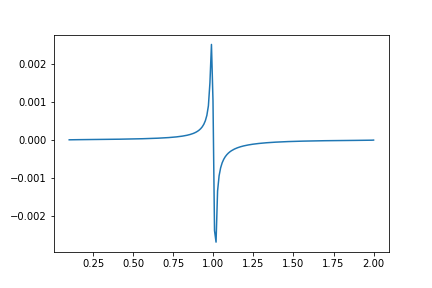
\includegraphics[width=0.7\linewidth]{one_site_secdev}
	\caption{Second Derivative Ergotropy ($g_0$)}
	\label{fig:onesitesecdev}
\end{figure}

\section{Two sites}

Eigenvalues of the correlation matrix
\begin{equation}
	\nu_{\pm}=\sqrt{\left(\frac{g_{1}-g_{-1}}{2}\right)^{2}+g_{0}^{2}} \pm \left| \frac{g_{1}+g_{-1}}{2} \right|
\end{equation}
$\nu_-<\nu_+$\\
\begin{figure}[h]
	\centering
	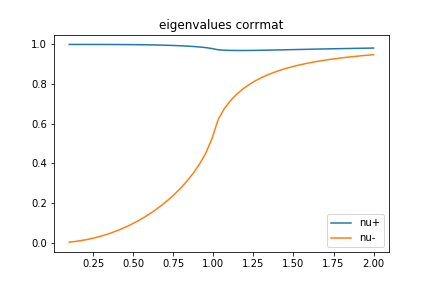
\includegraphics[width=0.7\linewidth]{nuplot}
	\caption{}
	\label{fig:nuplot}
\end{figure}
\begin{equation}
	\left\langle\hat{c}_{m} \hat{c}_{n}\right\rangle=0, \quad\left\langle\hat{c}_{m}^{\dagger} \hat{c}_{n}\right\rangle=\delta_{m n} \frac{1+\nu_{m}}{2}
\end{equation}
\begin{equation}
	\left\langle g\left|c_{j}^{\dagger} c_{j}\right| g\right\rangle=\frac{1+\nu_{j}}{2}
\end{equation}
Eigenvalues of the density matrix:
\begin{equation}
	p_{\pm \pm } =(1 \pm \nu_-)(1 \pm \nu_+)/4
\end{equation}
\begin{figure}[h]
	\centering
	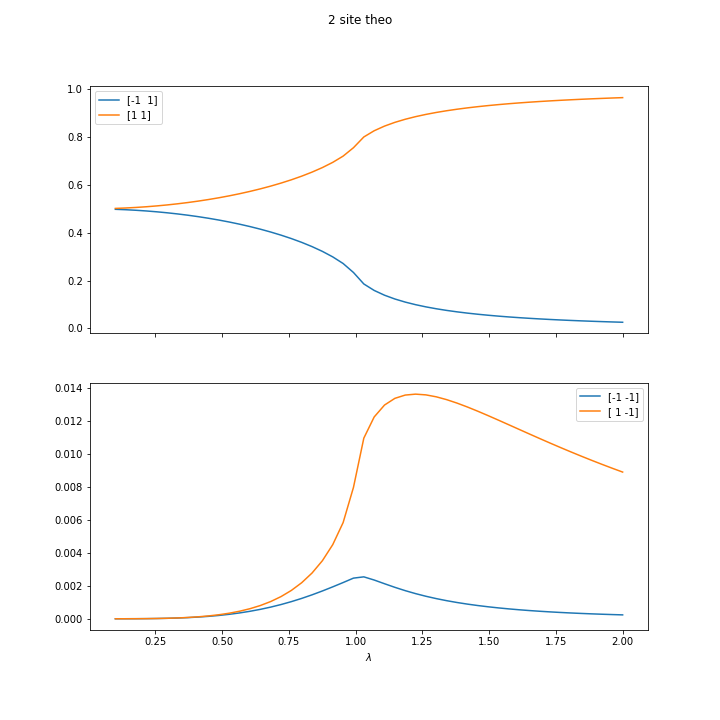
\includegraphics[width=0.7\linewidth]{two_site_theo}
	\caption{Eigenvalues of the 2-site density matrix}
	\label{fig:twositetheo}
\end{figure}

Eigenvalues of 2 site Hamiltonian:
\begin{equation}
	H=-\frac{1}{2} \left(\sigma^{x} \sigma^{x}+\lambda\sigma^{z} \sigma^0+\lambda\sigma^0\sigma^{z}\right) =
	\left(
	\begin{array}{cccc}
		-\lambda  & 0 & 0 & -\frac{1}{2} \\
		0 & 0 & -\frac{1}{2} & 0 \\
		0 & -\frac{1}{2} & 0 & 0 \\
		-\frac{1}{2} & 0 & 0 & \lambda  \\
	\end{array}
	\right)
\end{equation}
\begin{equation}
	\left\{-\frac{1}{2} \sqrt{1+4 \lambda ^2},-\frac{1}{2},\frac{1}{2},,\frac{1}{2} \sqrt{1+4 \lambda ^2}\right\}
\end{equation}

\begin{equation}
	\begin{aligned}
		&
		\mathcal{M}(\mathcal{I})=2 \sum_{i=1}^ {2}\left(p_{i}^{(\downarrow)}-p_{D-i+1}^{(\downarrow)}\right)\left|\epsilon_{i}^{(\uparrow)}\right|	\\
		& \left(p_{1}^{(\downarrow)}-p_{4}^{(\downarrow)}\right)\left|\epsilon_{1}^{(\uparrow)}\right|+\left(p_{2}^{(\downarrow)}-p_{3}^{(\downarrow)}\right)\left|\epsilon_{2}^{(\uparrow)}\right|=\\
		& (1/4)\left[(1+\nu_-)(1+\nu_+)-(1-\nu_-)(1-\nu_+)\right] \left(\sqrt{1+4 \lambda ^2}\right) + \\
		&(1/4)\left[(1-\nu_-)(1+\nu_+)-(1+\nu_-)(1-\nu_+)\right] = \\
		&\frac{(\nu_+ + \nu_-)}{2}\left(\sqrt{1+4 \lambda ^2}\right)+\frac{\nu_+-\nu_-}{2} \\
	\end{aligned}
\end{equation}
Normalized:
\begin{equation}
	\mathfrak{M}(\mathcal{I}) = \frac{\mathcal{M}(\mathcal{I})}{2\left|\epsilon_{1}^{(\uparrow)}\right|} =\frac{(\nu_+ + \nu_-)}{2}+\frac{(\nu_+-\nu_-)} {2\left(\sqrt{1+4 \lambda ^2}\right)}
\end{equation}
\begin{figure}[h]
	\centering
	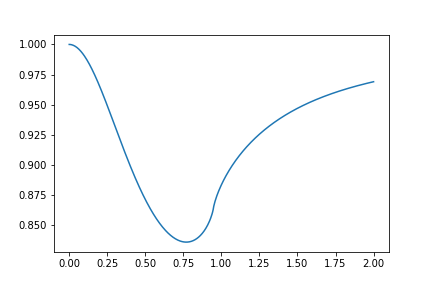
\includegraphics[width=0.7\linewidth]{2_site_ergo_theo}
	\caption{2 Site Max-Ergotropy}
	\label{fig:2siteergotheo}
\end{figure}
\begin{figure}[h]
	\centering
	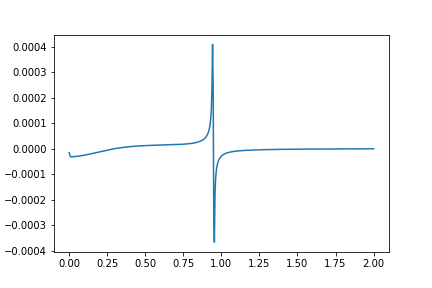
\includegraphics[width=0.7\linewidth]{2_site_ergo_theo_secdev}
	\caption{Second derivative 2 site Max-Ergotropy}
	\label{fig:2siteergotheosecdev}
\end{figure}
%Devi portare a 0 l'energia mi sa
\clearpage


\subsection{Two distant sites}
Let's try substituting $g_1$ with $g_d$ with d distance between sites.
Eigenvalues of the correlation matrix as in (PHYSICAL REVIEW A 78, 052302 2008)
\begin{equation}
	\nu_{\pm}=\sqrt{\left(\frac{g_{d}-g_{-d}}{2}\right)^{2}+g_{0}^{2}} \pm \left| \frac{g_{d}+g_{-d}}{2} \right|
\end{equation}
Eigenvalues of the density matrix:
\begin{equation}
	p_{\pm \pm } =(1 \pm \nu_-)(1 \pm \nu_+)/4
\end{equation}
Eigenvalues of distant Hamiltonian:
\begin{equation}
	H_{dist}=-(\lambda/2)(\sigma^z_l\sigma^0_{l+d} +\sigma^0_l\sigma^z_{l+d})
\end{equation}
\begin{equation}
	\text{eigs}= \{-\lambda,0,0 ,\lambda \}
\end{equation}
Normalized-Max-Ergo: (the two eigenvalues of the Hamiltonian are the same, so we simplify)
\begin{equation}
	\mathfrak{M}(\mathcal{I}) =	  \sum_{i=1}^ {2}\left(p_{i}^{(\downarrow)}-p_{D-i+1}^{(\downarrow)}\right) =	\frac{(\nu_+ + \nu_-)}{2}+\frac{(\nu_+-\nu_-)} {2}
\end{equation}




\chapter{Numerical Simulations}
\section{Exact Diagonalization}
\section{DMRG}

\chapter{Conclusions}
\end{document}
